%%%%%%%%%%%%%%%%%%%%%%%%%%%%%%%%%%%%%%%%%%%%%%%%%%%%%%%%%%%%%%%%%%%%%%
%
% レポートテンプレート
%
% updated 22 Oct, 2018
% last updated 02 Apr, 2021
%
% (c) Tohru TAKADA@UEC
% 各自のレポートに合わせて変更して使ってください.上記の行は残して使うこと.
% 2次配布可です.ご利用は計画的に.
%
%%%%%%%%%%%%%%%%%%%%%%%%%%%%%%%%%%%%%%%%%%%%%%%%%%%%%%%%%%%%%%%%%%%%%%

\documentclass[a4paper, 10pt]{jarticle}
\usepackage[dvipdfmx]{graphicx}
\usepackage{amsmath}
\usepackage{latexsym}
\usepackage{url}
\setlength{\textwidth}{165mm} %165mm-marginparwidth
\setlength{\marginparwidth}{40mm}
\setlength{\textheight}{225mm}
\setlength{\topmargin}{-5mm}
\setlength{\oddsidemargin}{-3.5mm}

\def\vector#1{\mbox{\boldmath $#1$}}
\newcommand{\AmSLaTeX}{%
 $\mathcal A$\lower.4ex\hbox{$\!\mathcal M\!$}$\mathcal S$-\LaTeX}
\newcommand{\PS}{{\scshape Post\-Script}}
\def\BibTeX{{\rmfamily B\kern-.05em{\scshape i\kern-.025em b}\kern-.08em
 T\kern-.1667em\lower.7ex\hbox{E}\kern-.125em X}}
\newcommand{\pderiv}[2]{{\partial#1\over\partial#2}}
\newcommand{\deriv}[2]{{{\rm d}#1\over{\rm d}#2}}
\newcommand{\dderiv}[2]{{{\rm d}^2#1\over{\rm d}#2^2}}
\newcommand{\DeLta}{{\mit\Delta}}
\renewcommand{\d}{{\rm d}}
\def\wcaption#1{\caption[]{\parbox[t]{100mm}{#1}}}
\def\rm#1{\mathrm{#1}}
\def\tempC{^\circ \rm{C}}

\makeatletter
%\def\section{\@startsection {section}{1}{\z@}{-3.5ex plus -1ex minus % -.2ex}{2.3ex plus .2ex}{\Large\bf}}
\def\section{\@startsection {section}{1}{\z@}{-3.5ex plus -1ex minus
-.2ex}{2.3ex plus .2ex}{\normalsize\bf}}
\makeatother

\makeatletter
\def\subsection{\@startsection {subsection}{1}{\z@}{-3.5ex plus -1ex minus
-.2ex}{2.3ex plus .2ex}{\normalsize\bf}}
\makeatother

\makeatletter
\def\@seccntformat#1{\@ifundefined{#1@cntformat}%
   {\csname the#1\endcsname\quad}%      default
   {\csname #1@cntformat\endcsname}%    enable individual control
}
\makeatother


%このようにパーセントを打つと,その行はコメントになります.メモ書きに使えますよ!

%%%%%%%%%%%%%%%%%%%%%%%%%%%%%%%%%%%%%%%%%%%%%%%%%%%%%%%%%%%%%%%%%%%%%%
\begin{document}

%
%% 通常は指定の表紙を付けて印刷して提出していますが,電子データをアップロードする際は
%% 表紙は付けなくても結構です.冒頭にタイトル,所属,学籍番号,氏名と記載日
%% 修正版を提出する際は更新日を書いてください
%
\begin{center}
{\Large{\bf レポートのためのテンプレート}} \\
{\bf 電気通信大学 1類1クラス\\
2311009 アハメドアティフ} \\
{\bf 2023年10月6日作成} \\
{\bf 2023年10月6日更新}
\end{center}
%%%%%%%%%%%%%%%%%%%%%%%%%%%%%%%%%%%%%%%%%%%%%%%%%%%%%%%%%%%%%%%%%%%%%%
\section{目的}

 実験の目的は,常にその課題で最終的に求める物理量について,「ooを求める.」といった
書き方をすると良いでしょう.基礎科学実験Aでは「重力加速度の測定」では「重力加速度を
4桁の精度で求める」ことが目的ですし,音の共鳴では「気体や固体中の波の速さ(音速)」を
求めること,「液体の比熱」では「水ならびにアルコールの比熱を加熱法と冷却法によって求める」
ことが目的です.

しかし,目的(続く節でも同様ですが)のセクションにこれだけ(骨格部分のみ)を書いただけでは,
貴方の文章を読んだ読者はこのレポートが無味乾燥でつまらないと思うことでしょう.
ですので,骨格部分に不必要に冗長的にならない程度に枝葉を付けていくことが必要です.
例えば,目的とする量はいったいどのようなものなのか,私たちの世界ではどういった役に
なっているのか,それを調べるとどのようなことが情報として得られるのか,こういったことを
調べて付加えると良いでしょう.

\vspace{3mm}
レポートは,このテンプレートが示すように「セクション構成」にします.各セクションはセクション番号と
セクション見出しを付け「ゴシック体」にして表します.本文は明朝体にしておきます.セクション見出しと
本文は同じフォントサイズを用いるので構いません.少なくとも本文に対してあまりにも大きい
フォントサイズにはしない方が無難です.このテンプレートのソースを見れば,\LaTeX についての
基本的な文法(数式を書くときや図の挿入方法,表の作成方法,参考文献の作り方等々)に
ついてどのように書けばどうなるのかが分かるはずです.テンプレートには出来上がりの
PDFもつけてありますので,よく見比べてください.テンプレートを使うときは必ず別名で
保存してから修正をすることを薦めます.


%%%%%%%%%%%%%%%%%%%%%%%%%%%%%%%%%%%%%%%%%%%%%%%%%%%%%%%%%%%%%%%%%%%%%%%
\section{原理}
実験の原理では目的に掲げた求めるべき物理量をどのような物理法則に基づいて求めるのかに
ついて数式を用いて解説します.皆さんが行う測定は,どのような数学的なモデルに
従って分布するのか,この原理のセクションで全て説明がされており,この意味ではどのような
結果を得るのかすでに判明しています.

例えば重力加速度では振子の等時性の式に対して半径が $r$ の剛体球を用いること,および
振子の振れ角が有限の $\theta$ という大きさであることの補正を取り入れた次式が用いられます.
%
\begin{equation}
T=2\pi \sqrt{\frac{h}{g}\left (1+\frac{2r^2}{5h^2}\right )} \times \left (1+\frac{\theta^2}{16}\right )
\label{grav_eq}
\end{equation}

実験の原理では上式で原理を終えるのは良い方法ではありません.なぜなら,あなたが
求めるべき量は重力加速ですから,式(\ref{grav_eq})を $g$ について解いた
ものを載せるのが良い方法です.

\begin{equation}
g=\frac{4\pi^2 h}{T^2}\times \left (1+\frac{2r^2}{5h^2} +\frac{\theta^2}{8}\right )
\label{grav2_eq}
\end{equation}

一行独立に書いている式には必ず式番号を割り振ってください.式のインデントの付け方は
分野によって幾つか流儀があるようです.物理では式を中央寄せ,数式番号は右寄せに
して行をそろえるのが一般的です.

\vspace{3mm}
\TeX では数式にはラベル(\verb|\label{<label>}|)を付けておき,後で参照(\verb|\ref{<label>}|)すると
式番号を自動的に引用します(後で途中に式を追加してもいちいち付け直す必要はありません).
ただし,引用は一度のコンパイルでは解決できない場合があります(??のように式番号が未定に
なります.メッセージを読むと警告が表示されているはずです).このようなときは
もう一度コンパイルをしてください.また,式をコピペしているときに起こりがちですが,ラベルは重複して
用いることはできません.ペーストした際はラベルを書き換えることを忘れないでください.

数式を書くのは \TeX に慣れるまでは存外面倒なものです.各課題について代表的な数式を
ここで掲載しておきましょう.どのように数式コマンドを書けばよいかの参考にしてください.

\subsection{重力加速度の測定}
不確かさを求める式は次のようになります.
\begin{eqnarray}
\overline{g}=\cfrac{\cfrac{g_1}{(\Delta g_1)^2}+\cfrac{g_2}{(\Delta g_2)^2}+\cdots+\cfrac{g_n}{(\Delta g_n)^2}}{\cfrac{1}{(\Delta g_1)^2}+\cfrac{1}{(\Delta g_2)^2}+\cdots+\cfrac{1}{(\Delta g_n)^2}} \\
\label{eq1}
\Delta g = \cfrac{1}{\sqrt{\cfrac{1}{(\Delta g_1)^2}+\cfrac{1}{(\Delta g_2)^2}+\cdots+\cfrac{1}{(\Delta g_n)^2}}}
\label{eq2}
\end{eqnarray}

\subsection{音の共鳴}
固体中の波の速さ $v_m$ に対する合成標準不確かさを求める式.
\begin{equation}
\frac{\Delta v_m}{v_m}=\sqrt{\left (\frac{\Delta L_g}{L_g}\right )^2+\left (\frac{\Delta l_m}{l_m}\right )^2+\left (\frac{\Delta v_g}{v_g}\right )^2}
\label{eq3}
\end{equation}

\subsection{液体の比熱}
加熱法による液体試料の温度上昇と時間の関係を表す式.
\begin{equation}
\frac{\Delta T}{\Delta t}=\frac{Ri^2}{MC+mc}
\label{eq4}
\end{equation}

\subsection{2次元の等電位線}
中央に導体がある等電位線の理論式の作図に関する式.
\begin{equation}
x=\pm \sqrt{\frac{y(-y^2+cy+R^2)}{y-c}}
\label{eq5}
\end{equation}

\subsection{電気回路}
抵抗,コイル,コンデンサの直列回路による過渡応答の原理式.
\begin{equation}
\dderiv{I(t)}{t}+2\gamma \deriv{I(t)}{t}+\omega_0^2I(t)=0
\label{eq6}
\end{equation}

ここで用いている\verb|\ddereiv|や\verb|\deriv|はこのファイルの冒頭に定義してあるもので,通常の
\TeX のコマンドではないことに注意が必要です.

\subsection{ヤング率}
たわみによるヤング率を求める式.
\begin{equation}
E=\frac{g}{2}\frac{l^3 d}{a^3 br}\frac{m}{S-S_0}
\label{eq7}
\end{equation}

\subsection{粘性率}
ポアズイユの法則を表す式.
\begin{equation}
p_1-p_2=\left (\rho g\cos\theta -\frac{2\gamma}{al}\right )l
\label{eq8}
\end{equation}

\subsection{光のスペクトル}
Na線の D$_1$線とD$_2$線の波長.

 D$_1$線:589.592 nm \\
 
 ${\rm D_2}$線:588.995 $\rm{nm}$

 \vspace{2mm}
 上記は同じ表示になるものを異なる方法で表記しています.ただし\verb|\rm|のコマンドは
 このファイルの冒頭で再定義しており,\TeX の本来のコマンドとは異なる挙動をしています.
 
\subsection{エアトラックによる力学実験}
滑走体のエアトラック上の運動方程式を減速の平均の加速度 $\overline{a}$ と平均速度 $\overline{v}$ で記述した式.
\begin{equation}
\frac{\overline{a}}{g}=\mu \cos\theta +\left (\frac{\lambda}{mg}\right )\overline{v}+\left (\frac{\kappa}{mg}\right )\overline{v}^2\mp\sin\theta
\label{eq9}
\end{equation}

\subsection{放射線の計測}
放射性同位元素セシウム137のベータ崩壊様式.

\begin{equation}
  ^{137}_{\hspace{1.2mm}55}\rm{Cs} \rightarrow ^{137}_{\hspace{1.2mm}56}\rm{Ba} + \rm{e}^{-} +\overline{\nu}_{\rm{e}}
  \label{beta-colps}
  \end{equation}

%%%%%%%%%%%%%%%%%%%%%%%%%%%%%%%%%%%%%%%%%%%%%%%%%%%%

\section{方法}
 原理で目的とする物理量を求めるために利用する法則を数式で説明をしました.
実験はテストの問題と異なり,それに基づいて測定器や実験装置を用いて測定値を得ることに
なります.このセクションに続く「実験結果」のセクションでデータを羅列しても,
一体どのようにそれを
測ったのかを説明しなければ読者は理解することはできません.このセクション「実験方法」で
主に書く内容は,
測定装置としてどのようなものを用いたのか,また測定手法はどのようなものであったのかを
説明をになります.ここで注意して欲しいことは,
「測定手法」を説明する際に,手順を逐一全て(マニュアルのように)書く必要はないということです.
\footnote{
実験テキストは,これを読んだ皆さんが上手に測定をできるように細かい手順を
書いていますが,皆さんはそれを参照して測定を行い,その結果をレポートに
まとめているのですから,オウム返しに同じことを書く必要はないのです.
}
実験方法のセクションに書く内容は時と場合によって異なるので唯一これを書いておけば
大丈夫といった処方箋はありません.ただ実験授業で与える課題の範疇では各範囲は
それほど振れ幅はないく,良い訓練の機会となります.このセクションで書く内容の
ポイントとしては次のような事柄を押さえるつもりで記載すると良いでしょう.

\begin{itemize}
  \setlength{\itemsep}{-2mm}
   \item 測定上特に注意をした点(注意をしなければならなかった点)
   \item 測定装置で特に説明をしなければ何故,どのように測定値を取得したのか
       読者にわからない点
   \item 実験結果を再現するために必要な特別な手順や測定方法など
   \item 測定データを処理する際に利用したソフトウェアで特に記載が必要なもの
  \end{itemize}

  記載内容全般に渡って言えることですが,理工系の実験レポートの読者は任意の他者ではなく,
  同程度の知識を有していることを前提で,このため同じ分野の人間にとって常識となっていることや,
  暗黙の了解となっていることは説明することはありません.散見される例として,例えば電圧を
  測ることに対し,実験方法で次のような箇条書きをしたらどうでしょうか?
  %
  \begin{enumerate}
  \setlength{\itemsep}{-2mm}
   \item 電圧はディジタルマルチメーターを用いて測った
   \item まずディジタルマルチメーターの電源をONにした
   \item 次にメーターのプローブを電源端子に接続し$\cdots$
  \end{enumerate}
  
  電圧を測る手段はそう多くはなく,およそまず「ディジタルマルチメーター」を想像するでしょう.
  また電気製品は電源を入れなけば動作しないことは万人が知っていることですし,
  プローブの類を端子に接触させなければ測れないのも当然のことでしょう.
  
  実験方法のセクションでは,以上のようにまず実験装置の概略図を載せます.そして,本当に
  説明が必要なことだけを説明しするので十分なのです.装置の図は
  本当に簡単なものでよく(凝ったイラストやカラーを用いる必要はありません.直線,四角,円で
  書いたようなもので十部です),ただし説明したい箇所を漏らさずに記載します.なお,作図を
  する場合に \TeX では EPS という形式のファイルを扱う方が仕上がりがきれいに
  出来ます.INKSCAPE 等フリーのツールもありますので活用してください.

  \vspace{3mm}
  一例として「液体の比熱」について詳しい説明をしましょう.この実験は液体の比熱を
  加熱法と冷却法で求めます.液体試料は「恒温槽」に格納されます.この恒温槽は
  水道水を常に流し込み一定の温度に保つという大変シンプルなものですが,この
  「流水の温度」が測定最中に変化しないかは大変重要な問題です.このため,
  実験中は流水の温度(環境温度) $T_\rm{A}$ を何回か測定をします.
  
  液体試料は均一温度になるよう「常に攪拌」を行う必要があります.攪拌のやり方が
  乱暴であると液体試料は容器からこぼれてしまいます.いずれにしても加熱や冷却で
  質量は変化する可能性が高く,このため実験では「液体試料の質量」を測定の
  前後で必ず2回測ります.

  加熱は 5$\sim$6 $\rm{\Omega}$ のマンガニン線をコイル状にし,そこに電流を
流してジュール熱を発生させて熱源とします.マンガニン線が空気中に露出すると
焼損をする可能性が高く,往々にして(慎重に攪拌したとしても)マンガニン線が焦げて
しまったという事故が起こります.この際に重要なのはどの時点でそれが発生したかに
なります(実験開始直後であれば測定を中止してやり直した方が早く,2/3程度
データが取得出来ていればそのまま続けても良い可能性があります).そこで,
測定最中「電流値」に変動がないか度々チェックしていることが重要です.また,
焦げていた場合は事後に「抵抗値を再度測定」して大きな変化がないか
確認する必要もあります.

以上が液体の比熱(加熱法)のあらましです.では,この実験について「実験方法」を
どのように書けばよいでしょうか?上で「」で囲った部分は重要な(私が読者に説明したいと
考えた)ポイントです.そこで,次のような文章と装置の図を書くことにしましょう.

\vspace{3mm}
\hrulefill

この実験では以下のような装置(図\ref{apara}参照)を用いて測定を行った。
液体試料を入れた熱量計を恒温槽(流水で内部を一定に保っている)に設置し(
恒温槽の底面と熱量計はスペーサーで断熱されている),熱量計には攪拌棒などが
入った状態で加熱用の蓋または冷却用の蓋で上部がふさがれる.
%
\begin{figure}[ht]
\begin{center}
 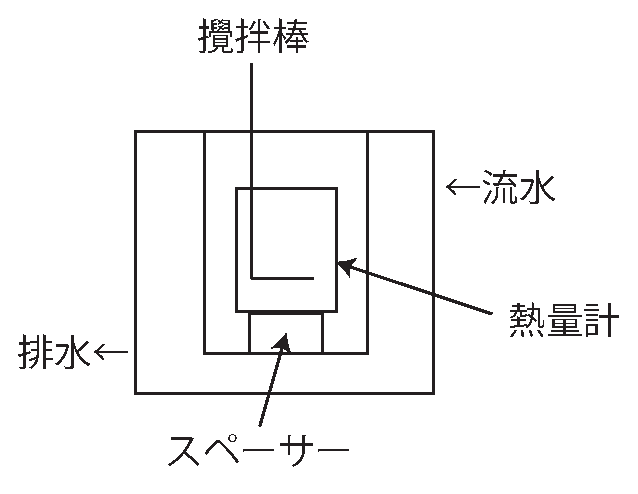
\includegraphics[scale=0.6]{aparatus2.eps}
 \caption{実験装置の概略図}
 %\ecaption{Options of documentclass.}
\label[apara]
\end{center}
\end{figure}


\end{document}

